% This is "sig-alternate.tex" V1.3 OCTOBER 2002
% This file should be compiled with V1.6 of "sig-alternate.cls" OCTOBER 2002

% NOTE: This document was modified by GMK starting on May 12, 2006

% For tracking purposes - this is V1.3 - OCTOBER 2002

\documentclass{sig-alternate}
\usepackage{url}

\usepackage{epsf}
\usepackage{upgreek}

\usepackage[named]{algo}

\begin{document}

%\conferenceinfo{PPPJ}{2006 Mannheim, Germany}

%%\title{Evaluating Java-Based Remote Communication Primitives}

% Note: the new title reflects a better understanding of the 
% word primitive -- it could be a data type of a communication tool

\title{An Empirical Comparison of Java Remote Communication Primitives
  for Intra-Node Communication}

%%\title{Evaluating Java Primitives Internode Communication}
%%\title{Can Java Primitives Support Communication \\in a Multi-Server
%%Operating System?}

\numberofauthors{1}
\author{
\alignauthor Philip F. Burdette, William F. Jones, \\
 Brian C. Blose, Gregory M. Kapfhammer \\
       \affaddr{Allegheny College}\\
       \affaddr{Department of Computer Science} \\ 
       \email{gkapfham@allegheny.edu}
}
%\date{2 May 2006}
\maketitle

\begin{abstract}

%% Response time results are also evaluated in light of metrics that
%% characterize the behavior of the Java virtual machine (JVM).

%% This is the first step towards determining if JVMs exhibit performance
%% characteristics that are amenable to the construction of multiserver
%% operating systems.

%% This paper presents a suite of micro benchmarks that
%% measure the performance of low-level socket-based primitives and
%% high-level remote communication with XML-RPC on the same computational
%% node with unique address spaces.  

%\vspace*{.05in}

%% This paper presents a suite of benchmarks that measure the performance
%% of the socket and eXtensible Markup Language remote procedure call
%% (XML-RPC) communication primitives when distinct address spaces
%% exchange messages while executing on the same computational node.

%% The Java programming language offers a wide variety of remote
%% communication primitives that vary according to their performance and
%% functionality.  

This paper presents a benchmark suite that measures the performance of
using sockets and eXtensible Markup Language remote procedure calls
(XML-RPC) to exchange intra-node messages between Java virtual
machines (JVMs).  The paper also reports on an empirical study
comparing sockets and XML-RPC with response time measurements from
profilers that use both operating system timers and Java language
instrumentation.  By employing packet filters within the GNU/\-Linux
kernel, the benchmark suite also calculates network resource
consumption.  Moreover, the framework interprets the response time
results in light of memory subsystem metrics characterizing the
behavior of the JVM.  The empirical findings indicate that sockets
perform better when transmitting small to very large objects, while
XML-RPC exhibits lower response time than sockets with extremely large
bulk data transfers.  The experiments reveal trade-offs in performance
and thus represent the first step towards determining if Java remote
communication primitives can support the efficient exchange of
intra-node messages.

%% that
%% is prevalent in modern systems.

%picking the best primitives for your application and its behavior characteristics

%The first 
%step towards determining if JVMs exhibit performance characteristics that
%are amenable to the construction of a multi-server OS.

%% can serve as valuable guides when selecting Java-based remote
%% communication primitives for use in a multi-server OS.

% NOTE: let's try this; remove this from the abstract and place 
% this kind of experiment summary information in the important 
% contributions listing

%% The empirical results indicate that Java programs which transmit large
%% parameters and return values can experience a 70\% increase in response
%% time when XML-RPC is used instead of sockets.  When compared to
%% sockets the XML-RPC primitive also exhibits greater response time
%% dispersion and thus has less predictable performance.  Use of the
%% benchmarking framework reveals that XML-RPC can consume 118\% more
%% network bandwidth than sockets and might be unsuitable for some
%% interactive Java applications.  The XML-RPC communication mechanism
%% requires additional time overhead to process the parameters that are
%% encoded as Strings.  This String processing causes the JVM that
%% executes the XML-RPC server to trigger one or more young garbage
%% collection (YGC) events.  In contrast, the socket-based server does not
%% require significant amounts of String processing and does not cause
%% any young GC events.

\end{abstract}

%\vspace*{-.1in}

%%\category{D.4.4}{Communications Management}{Message sending}
%%\category{D.4.7}{Organization and Design}{Distributed systems}
%%\category{D.4.8}{Performance}{Measurements}

%%\vspace*{-.1in}

%%\terms{Experimentation, Measurement, Performance}

%\vspace*{.05in}

%%\keywords{Java, sockets, XML-RPC, benchmarking}

\section{Introduction}
\label{sec:introduction}

%\vspace*{.05in}

%% Remote communication is used extensively in networked computers 
%% and distributed systems.  As the number of messages passed 
%% increases, it becomes increasingly important how much time and 
%% space overhead this communication requires.  

%% Remote communication performed in XML does not 
%% require either local or remote host to have the same operating 
%% system or for the different applications to be written in the 
%% same programming language.Socket communication operates at a lower 
%% level of abstraction.  

%% XML-RPC has become popular in the Java programming language because 
%% it makes implementing remote communication in programs much easier.  
				   
%% Remote Procedure Calls (RPCs) are designed to ensure that, within
%% limits, the invocation of a method on a remote computer is similar to
%% interprocess communication \cite{birrell-rpc}.

%%   A remote communication primitive can have a significant impact upon
%%   the functionality and performance of a distributed system. 

%% For instance, Herder et al.\ describe a multi-server operating system
%% that leverages several user-mode servers to create a reliable and
%% self-repairing operating system called MINIX 3
%% \cite{tanenbaum-minix3,herder-microkernel}.

Waldo et al.\ describe a category of ``local-remote'' object-based
systems where objects are in different address spaces but are
guaranteed to be on the same computational node \cite{waldo-note}.
Initially exemplified by systems such as Spring \cite{radia-spring}
and Clouds \cite{dasgupta-clouds}, these local-remote systems have
become increasingly prevalent, thus highlighting the need for
efficient intra-node communication primitives.  With the emergence of
powerful multi-core processors
\cite{lowney-multi-core,schalnsker-multi-core}, it may be desirable to
construct an efficient local-remote system from the servers that
previously executed in a distributed fashion.  In an attempt to
develop a highly reliable operating system, a local-remote approach
could leverage many user-mode servers that support self-repair
operations \cite{tanenbaum-minix3,herder-microkernel}.  Moreover,
efficient run-time debugging, profiling, and instrumentation
techniques often perform intra-node communication with the executing
program \cite{binder-instrument,wallace07superpin}.  While these types
of local-remote systems are often useful, flexible, and reliable, they
can incur increases in source code complexity and implementation
effort due to the use of custom intra-node communication primitives
\cite{tanenbaum-minix3,tang-code-complex,vaidyanathan-grid}.

%% We have chosen to run both JVMs on the
%%   same node due to the emergence of multiserver oprating systems,
%%   performance profilers, and debuggers \cite{dasgupta-clouds,
%%     tanenbaum-minix3, khalidi-spring}. 

%% Through the emergence
%%   of multi-core processors there is a need to re-evaluate these
%%   findings in order to enrich the knowledge of intra-node
%%   communication.

% Note: stress that Java provides a wide variety (no need to place it 
% in contrast per se) and say none just for intra-node probably first

\begin{sloppypar}
In contrast to specialized implementations of local-remote
communication, the Java programming language furnishes a wide variety
of remote communication primitives (RCPs) that have different
performance characteristics and functionality.  Yet, the Java
implementation of two representative RCPs, sockets and eXtensible
Markup Language remote procedure call (XML-RPC), were not specifically
designed to support communication between Java virtual machines (JVMs)
on the same computational node.  While previous empirical studies
suggest that sockets may perform up to an order of magnitude faster
than XML-PRC when transferring a significant amount of data across
nodes \cite{allman-per}, there is a relative dearth of information
about how these primitives support intra-node communication.
\end{sloppypar}

\begin{sloppypar}
To this end, this paper describes a benchmarking framework that uses
both Java language and operating system profilers, kernel packet
filters, and JVM behavior monitors to respectively characterize the
response time, network resource consumption, and memory subsystem
activity of both sockets and XML-RPC. In particular, the benchmarks
support the performance evaluation of Java-based software systems that
perform intra-node communication, as depicted in
Figure~\ref{fig:intranode-communication}.  The experimental results
indicate that the combined use of simple benchmarks and statistical
analysis techniques can identify important trade-offs in the
intra-node communication performance of Java programs.  

As such, this paper frames and begins to answer the question {\em can
  Java RCPs support intra-node communication}?  We anticipate that the
use of these benchmarks will develop a deeper understanding of Java's
remote communication primitives and subsequently lead to decreases in
the message passing overhead, code complexity, and implementation
effort associated with future local-remote systems that are developed
in the Java programming language.  In summary, the important
contributions of this paper include: \vspace*{-.1in}
\end{sloppypar}

%% This paper presents a benchmarking framework that
%% includes micro and macro benchmarks that measure the performance of
%% socket-based and XML-RPC intra-node communication.  The use of this
%% framework yields detailed quantitative results that characterize how
%% and why sockets and XML-RPC consume time overhead and network
%% bandwidth.

%%Through the emergence of of mutli-core
%%processors, performance evaluation of single node communication  

\begin{enumerate}

\setlength{\itemsep}{0in}
 \setlength{\topsep}{0in}
 \setlength{\partopsep}{0in}

\item A benchmarking framework that evaluates the performance of Java
  remote communication primitives and provides the following key
  features (Sections~\ref{sec:benchmark-framework} and
  \ref{sec:exper-goals-design}):

\begin{enumerate}

\setlength{\itemsep}{0in}
 \setlength{\topsep}{0in}
 \setlength{\partopsep}{0in}

%% \item Nano and macro benchmarks that can vary the size of the method
%%   parameters and return values.  The micro benchmarks establish
%%   baseline performance results for sockets and XML-RPC whereas the
%%   macro benchmarks mimic real programs by performing server
%%   computations (Section~\ref{sec:benchmark-framework}).

\item A suite of benchmarks with different types of computations and
  input and output sizes.

\item Variable granularity response time measurement with operating
  system and Java language timers.

\item The integration of the HotSpot\texttrademark Java virtual
  machine monitoring and measurement infrastructure so that response
  time can be explained in light of memory subsystem behavior.

\item The use of standard network packet capture tools to measure the
  consumption of network resources.

%% \item The use of the benchmarking framework in an execution
%%   environment that incorporates: (i) Java programming language version
%%   1.5.0 (ii) XML-RPC version 2.0 from the Apache Software Foundation,
%%   and (iii) GNU/Linux Kernel 2.6.12-1.1372 (Section~\ref{sec:design}).

\item Support for recent versions of Java sockets, XML-RPC, and the
  GNU/Linux operating system.

\end{enumerate}

\item Empirical results that reveal fundamental trade-offs in response
  time when remote communication primitives transfer data between
  client and server JVMs running on the same computational node
  (Section~\ref{sec:results}).
 
%% Additional string processing within the JVM of the XML-RPC server
%% triggers young garbage collection (YGC) events that lead to an
%% increase in response time and less predictable performance.  When
%% the socket server is used for bulk data transfer, the JVM performs
%% a significant number of YGC events that lead to severe performance
%% degradations

\end{enumerate}

%% \section{Motivation}
%% \label{sec:motivation}

%% Area for motivation content.

\section{Background}
\label{sec:background}

\subsection{Communication Primitives}
\label{sec:comm-prim}

% Goals for this paragraph: ``overview'' includes a discussion of when
% and where the communication primitive has been used

% 1. Overview of Sockets 
% 2. Overview of XML-RPC
% 3. There are some others (MPI, JavaSpaces, ...)
% 4. Why we focus on XML-RPC and sockets, allman and high vs low

%% Both sockets \cite{gagne-java-net} and XML-RPC
%% \cite{hansen-xml-events-guis} have also been integrated into the
%% computer science curriculum.

%% exist as alternatives to socket-based
%% and XML-RPC communication.  

The Java programming language provides a wide variety of RCPs that
could support the intra-node message exchange shown in
Figure~\ref{fig:intranode-communication}.  A local-remote system could
also use communication primitives such as the Java-Message Passing
Interface (Java-MPI) \cite{getov-mpi,judd-mpi-java}, Java remote
method invocation (RMI) \cite{grosso-rmi,maasen-java-rmi}, tuple
spaces \cite{arnold-javaspace-rdb,wells-linda-java-journal}, or JXTA
(i.e., ``Juxtapose'') \cite{oaks-jxta,seigneur-jxta}.  Yet, this paper
focuses on the performance evaluation of sockets and XML-RPC because
these primitives respectively represent (i) a low-level and a
high-level remote communication mechanism and (ii) a well established
standard and a recently proposed popular alternative.\footnote{{\small
    Since the benchmarking framework supports the integration of other
    RCPs, Section~\ref{sec:future-work} notes that we intend to
    incorporate and evaluate other communication primitives in future
    work.}} While sockets typically support high performance message
passing \cite{allman-per}, they may require a programmer to understand
several low-level implementation details.  Alternatively, XML-RPC
furnishes a high-level communication paradigm that enables programming
language independence and the rapid implementation of a program while
potentially compromising performance \cite{allman-per}.  Even though
the {\tt java.net} package provides a refined implementation of
sockets, XML can still be directly integrated into the Java
programming language \cite{harren-xj}.  Furthermore, XML-RPC libraries
are available for Java and systems such as OpenDHT use this protocol
to facilitate client communication \cite{rhea-opendht}.

The {\tt java.net.Socket} class provides an endpoint for communication
between two JVMs.  The {\tt bind} operation attaches a socket to a
local address on a computation node.  The {\tt accept} method blocks
the socket server until a connection from a client occurs and the {\tt
  connect} operation allows the client to actively seek out a server
at a specified address.  Sockets also furnish {\tt send} and {\tt
  receive} operations that enable the transmission of data.  Finally,
the {\tt close} method releases the socket's address and ensures that
it is not available for further data transmission.  Since there is
often a need for connection-oriented and reliable intra-node
communication, this paper evaluates the performance of socket-based
data transfer when TCP/IP governs the communication.

The XML-RPC primitive performs remote procedure calls that marshall
and unmarshall Java objects that are encoded in XML.  The Apache
XML-RPC 2.0 implementation provides a {\tt WebServer} class that is
instantiated on the side of the server and associated with a uniform
resource locator (URL).  All of the server's {\tt public} methods are
then available to clients through the {\tt WebServer} that handles the
XML parsing and local-remote communication.  The XML-RPC client is
responsible for creating an instance of the {\tt XmlRpcClient} class
that automatically binds to the server's URL. Finally, the client
invokes {\tt execute} with a textual description of the desired server
method and the Java objects that will serve as parameters.  This paper
measures communication performance when XML-RPC uses HTTP and TCP/IP,
due to the prevalence of this configuration.

\begin{figure}

\centering

\linethickness{1.1pt}
\frame{\begin{minipage}{2.5in}
\epsfig{file=intranode-communication-edited.eps} \vspace*{-.3in} \hspace*{.575in}
 \mbox {\bf Computational Node} \end{minipage} }

\vspace*{.3in}

\caption{Intra-Node Communication.}

\label{fig:intranode-communication}
\end{figure}

\subsection{Benchmark Suites}
\label{sec:benchmarking-suites}

% NOTE: this paragraph was changed so that the reader can tell that we
% are now focusing on nano and micro benchmarks.  I picked to use
% ``nano'' instead of ``kernel'' since we use kernel to have another
% meaning in the paper!

%% micro- (µ-)

%% 10-6

%% 1 millionth

%% nano- (n-)

%% 10-9

%% 1 billionth

\begin{sloppypar}
Zhang and Seltzer observe that there are three main purposes for
benchmarking: (i) comparing the performance of different systems, (ii)
guiding performance optimizations, and (iii) predicting an
application's performance in new software and hardware environments
\cite{zhang-hbenchjava}.  Furthermore, Zhang and Seltzer place
software performance benchmarks into one of four categories: (i)
micro, (ii) macro, (iii) combined, and (iv) application-specific
benchmarks \cite{zhang-hbenchjava}.  In the context of intra-node
communication, this paper describes nano and micro benchmarks that
measure the performance of remote communication primitives for Java.
Our nano benchmarks focus on the analysis of several basic operations
that are commonly used in local-remote applications (e.g.,
transmission of a single value or a list of data
values).\footnote{{\small Since the metric prefix ``nano'' ($10^{-9}$)
    denotes a number that is smaller than the one described by the
    ``micro'' ($10^{-6}$) prefix, we use the term {\em nano benchmark}
    to refer to a benchmark that is smaller than its macro
    counterpart.  We selected this descriptor instead of the
    previously used term {\em kernel benchmark} \cite{agarwal-sp2}
    since ``kernel'' now commonly refers to a part of an operating
    system. }}  The micro benchmarks incorporate small and
well-defined operations (e.g., finding a data value in a list or
reversing the provided list) that require server-side computations and
thus may be found in real-world local-remote systems.
\end{sloppypar}

According to Horgan et al. \cite{horgan-measure-runtime}, the
performance evaluation of Java programs can take place at four
different levels, namely (i) statically, with the source code; (ii)
statically, with the bytecode; (iii) dynamically, with the bytecode;
and (iv) dynamically, on a specific virtual machine and architecture.
This paper focuses on the fourth category by analyzing the performance
of Java-based RCPs on a specific JVM, computer architecture, and
operating system kernel. The performance measurements that result from
benchmark execution are further explained in light of JVM behavior
profiles.  Building on the insights developed by Heydon and Najork
\cite{heydon-java-core}, this paper also examines how excessive heap
allocation and the frequent execution of the garbage collector can
impact the performance of intra-node communication.

%% A micro benchmark for JavaSpaces could measure the performance of
%% basic space operations like {\tt read}, {\tt write}, and {\tt take}.

\vspace*{-.1in}

\section{Benchmarking Framework}
\label{sec:benchmark-framework}

%% Experiments are run in experimental campaigns.  The phases of a
%% campaign can be seen in Figure~\ref{fig:expdes}.  First, the benchmark
%% framework starts the server.  Then packet capture is started.  Next,
%% the client executes and then the framework waits to allow the server
%% to return to a quiescent state.  The client executes \texttt{i} times.
%% Following the client executions, the benchmark framework stops packet
%% capture.  The final step in the experiment is to stop the execution of
%% the server.

%%  and a communication parameter $V$.

Figure~\ref{fig:experiment-campaign} describes the {\em
  ExperimentCampaign} that executes $N$ trials of benchmark $B$ when
it is configured to use communication primitive $P$. Line~\ref{init}
of Figure~\ref{fig:experiment-campaign} respectively initializes the
sequences (i.e., ordered tuples) of response times ($\mathcal{R}$),
network resource consumptions ($\mathcal{W}$), and JVM behavior
profiles ($\mathcal{J}$) so that they can be populated with
measurements during the execution of the experiments.  The socket or
XML-RPC server starts on line~\ref{start} and then the framework
pauses so that the server can enter a quiescent state and the packet
capture tool can initialize.  Lines~5 through~\ref{pause2} ensure that
(i) benchmark $B$ executes for $N$ trials, (ii) the response time and
JVM profiles are properly stored for later analysis, and (iii) the
server pauses in preparation for the next benchmark trial.  These
lines use the order preserving union operator, denoted $\uplus$, to
add data values to $\mathcal{R}$ and $\mathcal{J}$.  In an attempt to
minimize the startup time of the framework, the server and the packet
capture tool run continuously for the duration of the $N$ trials
(exploratory experiments indicated that all of the empirical results
were not sensitive to this optimization).  Finally, {\em
  ExperimentCampaign} terminates when line~\ref{return} returns the
evaluation metrics.

\begin{figure}

%% \centering
%% 
\epsfig{file=phases.eps}
%% \caption{Experiment Campaign Design}\label{fig:expdes}

 \begin{center}
      \begin{algorithm}{ExperimentCampaign}[B, P, N]
        { \qinput{Benchmark $B$; \newline 
	    \hspace*{.16in} Communication Primitive $P$; \newline
            %\hspace*{.16in} Communication Vector $V$; \newline
            \hspace*{.16in} Number of Experiment Trials $N$;}
	  \qoutput{Response Time Sequence $\mathcal{R}$; \newline
            \hspace*{.26in} Network Consumption Sequence $\mathcal{W}$; \newline
	    \hspace*{.26in} JVM Profile Sequence $\mathcal{J}$}
        } 
    $\mathcal{R} \qlet \emptyset; \; \mathcal{W} \qlet \emptyset; \; \mathcal{J} \qlet \emptyset$; \label{init}\\	
    \mbox{{\em StartServer}}$(B,P)$ \label{start}\\
    \mbox{{\em Pause()}} \label{pause1} \\
    \mbox{{\em StartPacketCapture}}$(B,P)$ \label{packstart} \\
    \qfor $i \in \{1, \ldots, N\}$ \label{for} \\
    \qdo $\{R(B,P), J(B,P)\}$ \qlet \mbox{{\em Execute}}$(B,P)$ \label{exec} \\
    $\mathcal{R} \qlet \mathcal{R} \uplus \langle R(B,P) \rangle$ \label{storeR} \\
    $\mathcal{J} \qlet \mathcal{J} \uplus \langle J(B,P) \rangle$ \label{storeJ} \\
    \mbox{{\em Pause()}} \label{pause2} \qrof \\
    \mbox{{\em StopServer}}$(B,P)$ \label{stop} \\  
    $W(B,P)$ \qlet \mbox{{\em StopPacketCapture}}$(B,P)$ \label{packstop} \\
    $\mathcal{W} \qlet \langle W(B,P) \rangle$ \label{storeW} \\
    \qreturn $\mathcal{R},\mathcal{W},\mathcal{J}$ \label{return}
  \end{algorithm}
  \end{center}
\vspace*{-.15in}
\caption{The {\em ExperimentCampaign} Algorithm.}

\label{fig:experiment-campaign}
\vspace*{-.2in}
\end{figure}

% NOTE: This has been changed to refer to nano benchmarks!

Table~\ref{tab:baselines} lists the four nano benchmarks that are
similar to those that are described by Allman \cite{allman-per}. These
nano benchmarks perform minimal computation on the side of the server
in order to provide a baseline for the response time measurements.
The \texttt{SS} benchmark uses a client that sends and receives a
single data value, which is either an integer or a string.  The client
for \texttt{SV} sends a single data value and receives a vector of
values.  The \texttt{VS} benchmark has a client that sends a vector of
values and receives a single value.  Finally, the \texttt{VV}
benchmark causes the client to send and receive a vector of data
values.  During {\em ExperimentCampaign} the size of the vector of
values, denoted $size(V)$, is fixed throughout every execution trial
of {\tt SV}, {\tt VS}, and {\tt VV}.

% NOTE: Argh!  This means that this has to be a parameter to the algorithm
% But, that seems forced and I have removed it again (Brian, help)

%% all $L$ executions experiments within a campaign and is set to a
%% specific value.  The default size of the vector is five objects.

%% which sends a single Integer to the server.  The server has an Array
%% of Integers created during startup, and returns the Integer at the
%% Array index of the Integer sent by the client.

%% The server finds the greatest common divisor and then returns that
%% Integer.

%% The \texttt{FIND} benchmark is initialized with a vector of integers
%% and the client transmits a single integer to the Server.

%% return the value that was stored vector index that contains the
%% client's integer and thus it is of

This paper also uses the four micro benchmarks listed in
Table~\ref{tab:realworlds}.  After \texttt{GRAB}'s server randomly
generates a vector of integers, the client transmits a single integer
to the server.  This benchmark is of type {\tt SS} since we configured
the {\tt GRAB} server to use the client's integer as an index into its
vector and subsequently return the resulting integer.  {\tt FACT} is
an {\tt SV} benchmark because it sends an integer value to a server
that enumerates all the factors of the integer and returns a vector of
integers.  The type {\tt VS} benchmark called {\tt GCD} sends a vector
of integers to a server that calculates the greatest common divisor
and returns this integer to the client.  The final benchmark is
\texttt{REV}, which sends a vector of integers to the server.  This
benchmark is of type {\tt VV} because the server reverses the order of
the elements within the vector and returns this new vector back to the
client.

\section{Experiment Goals and Design}
\label{sec:exper-goals-design}

\subsection{Evaluation Metrics}
\label{sec:evmet}

\begin{table}[t]

  \begin{center}
  \begin{tabular}{| c | c | c |}
  \hline
  Experiment & Sent by client & Received by client \\
  \hline
  \texttt{SS} & Single value & Single value \\
  \texttt{SV} & Single value & Vector \\
  \texttt{VS} & Vector & Single value \\
  \texttt{VV} & Vector & Vector \\
  \hline
  \end{tabular}
\end{center}

  \vspace*{-.1in}
  \caption{Nano Benchmarks.}\label{tab:baselines}
  %\vspace*{.05in}

\end{table}

\begin{table}[t]

  \begin{center}
  \begin{tabular}{| c | c | c |}
  \hline
  Experiment & Sent by client & Received by client \\
  \hline
  \texttt{GRAB} ({\tt SS}) & Single value & Single value \\
  \texttt{FACT} ({\tt SV}) & Single primitive & Vector \\
  \texttt{GCD}  ({\tt VS}) & Vector & Single value \\
  \texttt{REV}  ({\tt VV}) & Vector & Vector \\
  \hline
  \end{tabular}
\end{center}

  \vspace*{-.1in}
  \caption{Micro Benchmarks.}\label{tab:realworlds}
  \vspace*{-.2in}

\end{table}

% content modified by gmk

% NOTE: probably not really needed

%% In order to describe the evaluation metrics this paper enhances the
%% notation established by Fiedler et al. \cite{fiedler-per}.

The primary goal of the experiments is to measure the time overhead
and network consumption associated with socket and XML-RPC
communication.  Equation~(\ref{eq:time}) defines $R(B,P)$, the
response time associated with the execution of a benchmark $B$ from
either Table~\ref{tab:baselines} or \ref{tab:realworlds} and a remote
communication primitive $P$ that is either sockets ($S$) or XML-RPC
($X$).  For instance, $R(\mbox{{\tt GCD}}, X)$ denotes the response
time for the execution of the {\tt GCD} benchmark with the XML-RPC
primitive.  Equation~(\ref{eq:time_change}) describes $R_\Delta
(B,P,P')$, the change in response time when we replace communication
primitive $P$ with primitive $P'$.  Next,
Equation~(\ref{eq:time_percent_incr}) defines {\small
  $R_\Delta^\%(B,P,P')$}, the percent change in response time when the
benchmark $B$ uses $P'$ instead of $P$.  For example, {\small
  $R_\Delta^\%(\mbox{{\tt FACT}},S,X)$} stands for the percent change
in response time when {\tt FACT} uses XML-RPC rather than sockets.
Since it is often useful to calculate how response time changes when
$P'$ replaces $P$ for a set of benchmarks designated $\upbeta$ (e.g.,
all of the micro benchmarks in Table~\ref{tab:realworlds}),
Equation~(\ref{eq:time_percent_incr_set}) characterizes {\small
  $R_\Delta^\%(\upbeta,P,P')$}, the average percent change in response
time over all of the benchmarks $B \in \upbeta$.

\vspace*{-.1in}

\begin{equation} \label{eq:time}
R(B,P) = \mbox{{\em T}}_{complete}(B,P) - \mbox{{\em T}}_{start}(B,P)
\end{equation}

\vspace*{-.1in}

\begin{equation} \label{eq:time_change}
R_\Delta (B,P,P') = R(B,P') - R(B,P)
\end{equation}

\vspace*{-.1in}

\begin{equation} \label{eq:time_percent_incr}
R_\Delta^\%(B,P,P')  = \frac{R_\Delta (B,P,P')}{R(B,P)} \times 100
\end{equation}

\vspace*{-.1in}

\begin{equation} \label{eq:time_percent_incr_set}
R_\Delta^\%(\upbeta,P,P')  = \frac{\displaystyle \sum_{B\in\upbeta} R_\Delta^\% (B,P,P')}
                          {|\upbeta|} 
\end{equation}

\begin{sloppypar}
The benchmarking framework measures response time with timers that
operate at two distinct levels of granularity.  We leverage the
operating system tool \texttt{/usr/bin/time} to record the coarse
granularity time overheads.  These operating system-based response
times include the time required to start the client, communicate with
the server, and shutdown the client.  The benchmarks use Java language
instrumentation within the client's source code to measure the fine
granularity response times.  The instrumentation records $\mbox{{\em
    T}}_{start}(B,P)$ before calling the server and then saves
$\mbox{{\em T}}_{complete}(B,P)$ after the server finishes the
computation.
\end{sloppypar}

\begin{sloppypar}
Unless specified otherwise, this paper always reports the change and
percent change in response time when the socket communication
primitive is replaced with XML-RPC.  For each of the benchmarks
described in Section~\ref{sec:benchmark-framework}, the results
analysis in Section~\ref{sec:results} always reports $R_\Delta(B,S,X)$
and {\small $R_\Delta^\%(B,S,X)$}.  A positive value for {\small
  $R_\Delta^\%(B,P,P')$} indicates an increase in $R(B,P)$ and a
negative value shows that response time decreased when benchmark $B$
uses primitive $P'$ instead of $P$.  The framework also use the {\tt
  jvmstat} and {\tt hprof} tools to generate each JVM behavior profile
in $\mathcal{J}$.  Finally, the benchmarking framework employs
Roubtsov's object sizing technique \cite{roubtsov-sizing} to calculate
the size of the method parameters and return values and, for each
benchmark $B$ and primitive $P$, it appends these values to the
appropriate profile in $\mathcal{J}$.
\end{sloppypar}

%% The first are from an operating system-based timer,
%% \texttt{/usr/bin/time}.  This timer encapsulates the call within the
%% benchmarking framework to run the client.

%% The operating system-based timer times the total execution 
%% of the client application, including startup time of the client.  

% NOTE: I don't think that this is needed because it is clear 
% by looking at the algorithm statement

%% Space overhead is collected for every ten executions of the client, or
%% for every execution of the server.

Even though our focus is on intra-node communication, the use of HTTP
and TCP/IP requires the client and server to transfer messages across
the network interface.  Therefore, we configured the \texttt{tcpdump}
tool to receive and attempt to record all of the packets that are
transmitted across the network interface and we use the {\tt capinfos}
tool to analyze the captured packets.  The data reported by {\tt
  tcpdump} and {\tt capinfos} includes the (i) total number of packets
received by the kernel filter, (ii) number of packets captured and
stored for later analysis, and (iii) average packet size.  Due to the
high rate of data transfer, the number of captured packets can be much
lower than the number of packets that were received by the {\tt
  tcpdump} filter.  Since \texttt{capinfos} can only analyze the
captured packets, it is not always possible to accurately measure the
total amount of network resources that the benchmark consumed during
execution.  

\begin{sloppypar}
The benchmarking framework estimates the total network consumption in
bytes, defined as $W(B,P, \Phi_c, \Phi_r)$ in
Equation~(\ref{eq:space_calculate}), by multiplying the average size
of the captured packets by the total number of packets received by the
{\tt tcpdump} filter.  Equation~(\ref{eq:space_calculate}) uses
$\Phi_c$ and $\Phi_r$ to respectively stand for the sets of captured
and received packets.  Moreover, this equation uses the {\em size}
function to return the size in bytes for a given packet $\upphi \in
\Phi_c$.  $W(B,P, \Phi_c, \Phi_r)$ is a only estimate of the actual
network consumption since it assumes that all packets that were
received, but not captured and analyzed, are of the average size of
those packets $\upphi \in \Phi_c$.  While the use of $W(B,P, \Phi_c,
\Phi_r)$ is a reasonable first step towards approximating network
consumption, Section~\ref{sec:future-work} suggests ways to avoid this
estimation of network resource consumption and thus improve future
empirical studies of Java's remote communication primitives.
\end{sloppypar}

\vspace*{-.1in}

\begin{equation} \label{eq:space_calculate}
W(B,P, \Phi_c, \Phi_r) = \frac{\displaystyle \sum_{\upphi \in \Phi_c}
                   \mbox{{\em size}}(\upphi)}
         {|\Phi_c|} \times |\Phi_r|
\end{equation}

% NOTE: I am not sure that this sentence will be needed anymore -- it
% may be, but only after I define another equation!

%% The change and percent change of the network consumption metric,
%% $W(B,P)$, can be defined in a fashion analogous to
%% Equations~(\ref{eq:time_change}) and~(\ref{eq:time_percent_incr}).

% NOTE: Re-writing the entire paragraph to better avoid passive voice

%% \begin{sloppypar}
%% Response time is measured with timers that operate at two different
%% levels of granularity.  The coarse granularity times are recorded by
%% the operating system tool \texttt{/usr/bin/time}.  The operating
%% system-based response times include the time required to start the
%% client, communicate with the server, and shutdown the client. The fine
%% granularity response times are measured by Java language
%% instrumentation within the client source code.  The invocation of the
%% server is enclosed by additional Java statements that record
%% $\mbox{{\em T}}_{start}(B,P)$ and $\mbox{{\em T}}_{complete}(B,P)$.
%% We also used the {\tt jvmstat} and {\tt hprof} tools to generate the
%% behavior profiles for the JVM and Roubtsov's object sizing technique
%% to measure the size of the method parameters and return values
%% \cite{roubtsov-sizing}.
%% \end{sloppypar}

% NOTE: this is residual content; did I summarize correctly?

%% upon the packets that were captured and generates an average packet
%% size.  Because the average packet size is not based on the total
%% number of packets received,

\vspace*{-.05in}
\subsection{Experiment Design}
\label{sec:design}

\begin{figure*}[t]
\centering
\begin{tabular}{c c}

\begin{minipage}{3.5in}
\centering
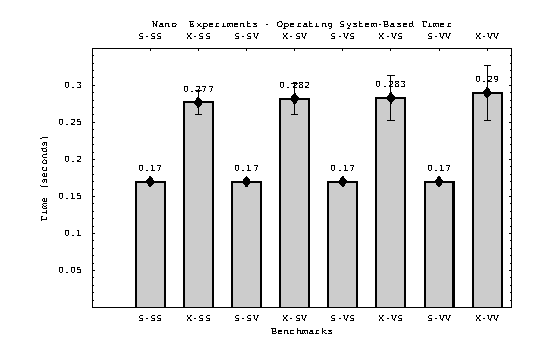
\epsfig{file=base_op.eps}
\vspace*{-.1in}
\begin{center}(a)\end{center}
\end{minipage} &

\begin{minipage}{3.5in}
\centering
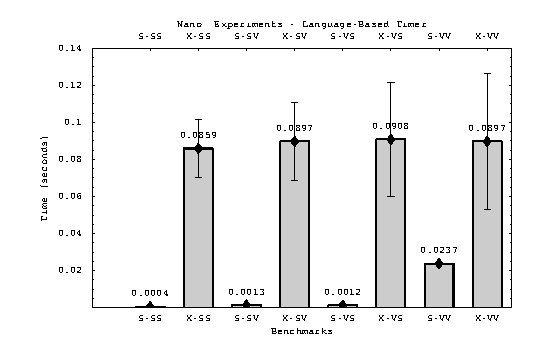
\epsfig{file=base_lang.eps}
\vspace*{-.1in}
\begin{center}(b)\end{center}
\end{minipage} \\

\end{tabular}

\vspace*{-.1in}
\caption{Nano Benchmarks Using the (a) Operating System-Based and (b)
Language-Based Timers.}\label{fig:baselines}
\vspace*{-.1in}
\end{figure*}

% explains what hyper-threading actually is; adds in a few more details

% Brian, is this L1 or L2 cache?  We need to be clear about this!

All experiments were conducted on a GNU/Linux workstation with kernel
2.6.12-1.1372, a dual-core 3 GHz Intel Pentium 4 processor, 1 GB of
main memory, and 1 MB of L1 cache.  The workstation used a Serial ATA
connection to the hard drive and CPU hyper-threading was enabled in
order to support thread-level parallelism.  The experiments use a JVM
version 1.5.0\_02 that was set to operate in Java
HotSpot\texttrademark client mode with a 64 MB heap.  Since our focus
is on intra-node communication, we ran the benchmark client and server
in separate JVMs on the same computational node.  If desired, the
benchmarking framework can be configured so that the client and server
execute on separate nodes.  We implemented XML-RPC communication with
Apache XML-RPC 2.0 and the socket-based benchmarks use the classes
provided by the {\tt java.net} package. For the results in
Section~\ref{sec:results}, we initialized {\em ExperimentCampaign} so
that $N=10$.  We also set $size(V) = 5$ in order to produce the
empirical results described in Section~\ref{sec:time-overhead}.

% NOTE: none of this content is needed because it was consolidated in
% the section that describes the benchmarking framework

%% We designed an experiment to measure the time and space overheads of
%% sockets compared to XML-RPC, using two groups of benchmarks.  The
%% micro benchmarks do not require a significant amount of processing on
%% the side of the server.  These benchmarks were designed to establish
%% the baseline communication costs associated with each remote
%% communication primitive.  The macro benchmarks involve a higher degree
%% of computation on the side of the server.  These benchmarks more
%% closely resemble actual situations utilizing remote communication.

Section~\ref{sec:results} analyzes the $N$ response time measurements
in $\mathcal{R}$ with descriptive statistics such as the arithmetic
mean, denoted $R_\mu (\mathcal{R}, B, P)$ and defined in
Equation~(\ref{eq:time_mean}).  Figures~\ref{fig:baselines}
through~\ref{fig:varying} graphically depict the value of
$R_\mu(\mathcal{R}, B,P)$ by the height of the corresponding bar.  We
also measure the dispersion of the $N$ response times in the sequence
$\mathcal{R}$ by calculating the standard deviation, designated as
$R_\sigma (\mathcal{R}, B, P)$ and defined in
Equation~(\ref{eq:time_stdev}).  The graphs in
Figures~\ref{fig:baselines} through~\ref{fig:varying} use an error bar
to demarcate the range of values in the closed interval
$[R_\mu(\mathcal{R}, B,P)-R_\sigma (\mathcal{R}, B, P),
  R_\mu(\mathcal{R}, B,P)+R_\sigma (\mathcal{R}, B, P]$. Finally,
Figures~\ref{fig:baselines} through~\ref{fig:varying} use a diamond to
signal that the value of $R_\sigma (\mathcal{R}, B, P)$ is too small
to graphically present at the top of a bar.

\vspace*{-.1in}

\begin{equation} \label{eq:time_mean}
R_\mu (\mathcal{R}, B, P) = \frac{\displaystyle \sum_{R(B,P) \in \mathcal{R}} R(B,P)}{|\mathcal{R}|}
\end{equation}

\begin{equation} \label{eq:time_stdev}
R_\sigma (\mathcal{R}, B, P) = 
      \sqrt{\frac{\displaystyle \sum_{R(B,P) \in \mathcal{R}} 
                                (R(B,P) - R_\mu (\mathcal{R}, B, P))^2}
                 {|\mathcal{R}|}}
\end{equation}


Whenever the remote communication primitives demonstrate performance
characteristics of the greatest similarity, we also calculate a mean
confidence interval and perform a mean difference hypothesis test.
Within a group of similar benchmarks $\upbeta$, we perform additional
statistical analysis for a benchmark $B \in \upbeta$ and the two
primitives $P$ and $P'$ whenever (i) $R(B,P') - R(B,P)$ is the
smallest or (ii) either $R(B,P')$ or $R(B,P)$ has the largest standard
deviation.  For instance, the results in Figure~\ref{fig:baselines}(a)
prompted us to compare (i) S-{\tt SS} to X-{\tt SS} because
$.277-.17=.107$ is the smallest difference between two benchmarks and
(ii) S-{\tt VV} to X-{\tt VV} since X-{\tt VV} shows the largest
standard deviation.  Table~\ref{tab:XMLResults} summarizes the
confidence intervals that we calculated.

%% Finally, Equation~(\ref{eq:time_mean}) gives $R_\mu (\mathcal{R}, B,
%% P, N)$, the arithmetic mean of the $N$ response time values for a
%% specific benchmark $B$ and a remote communication primitive $P$.

%\begin{sloppypar}

We apply these additional statistical analyses under the assumptions
that (i) the response times adhere to an interval measurement scale,
(ii) the $N$ samples within $\mathcal{R}$ are independent, and (iii)
the variances of the response times for the two different
communication primitives are not equal.  Assumption (i) is justified
because the difference between two response time measurements is
meaningful. That is, if response time is measured in seconds and we
have $R_1(B,P) = .15$ and $R_2(B,P) = .10$, then we can accurately say
that $R_1$ is .05 seconds slower than $R_2$.  We judge that assumption
(ii) is valid because {\em ExperimentCampaign} includes configurable
pauses between each execution trial of a benchmark (we set the pause
to five seconds for all of the empirical results in
Section~\ref{sec:results}, although this time period is a configurable
parameter of the framework).  Since the results also demonstrate that
the variances were not always exactly equal, as stated in assumption
(iii), we employ the Welch's approximate t-test rather than the
traditional t-test.

% that assumes equal variances.

%\end{sloppypar}

%% The framework calculates the CIs using the default configuration of
%% the Student's t-test implemented in the R language for statistical
%% computation \cite{crawley-rbook}.  

%% In fact, Table~\ref{tab:XMLResults} reveals that many of the resulting
%% confidence intervals are very tight.

For a benchmark $B$ and two remote communication primitives $P$ and
$P'$, we formulate the null hypothesis as $H_0: R_\mu(B,P) =
R_\mu(B,P')$.  A rejection of $H_0$ suggests that communication
primitives $P$ and $P'$ have different response time characteristics
and, all other factors being equal, we would prefer the primitive with
the lower response time values.  Since we configured the t-test with a
significance level of .01 (i.e., $\alpha=.01$), the data in
Table~\ref{tab:XMLResults} represents the 99\% confidence interval
(CI) for the arithmetic mean of the $N$ response times.  For each
response time mean in the confidence interval $[l, u]$, we can be
$99\%$ certain that the mean of the response time values from
subsequent experiments will fall between the lower bound $l$ and the
upper bound $u$.  Therefore, small confidence intervals suggest that
our benchmarking framework generates empirical outcomes in a
repeatable and predictable manner.

\begin{figure*}[t]
\centering
\begin{tabular}{c c}

\begin{minipage}{3.5in}
\centering
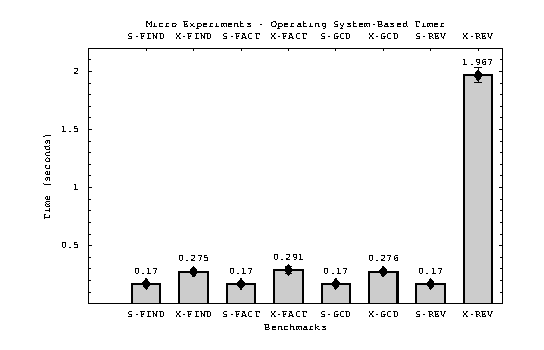
\epsfig{file=realworld_op.eps}
\vspace*{-.1in}
\begin{center}(a)\end{center}
\end{minipage} &

\begin{minipage}{3.5in}
\centering
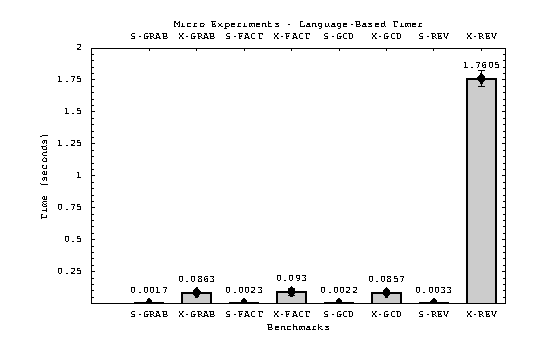
\epsfig{file=realworld_lang.eps}
\vspace*{-.1in}
\begin{center}(b)\end{center}
\end{minipage} \\

\end{tabular}

\vspace*{-.1in}
\caption{Micro Benchmarks Using the (a) Operating System-Based and (b)
Language-Based Timers.}\label{fig:realworlds}
\vspace*{-.1in}
\end{figure*}

%% For given class of benchmarks and timers (e.g., the micro benchmarks
%% and the language-based timers),

% NOTE: this is the listing of the high-level empirical results
% These were removed from the introduction of the paper since they
% did not fit well at this location.

%% \begin{enumerate}

%% \setlength{\itemsep}{0in}
%%  \setlength{\topsep}{0in}
%%  \setlength{\partopsep}{0in}

%% \item {\em Response Time}: When socket-based communication was
%%   replaced with XML-RPC, the benchmarks that use large parameters and
%%   return values experienced an increase in response time that ranged
%%   from $66\%$ to $313\%$ (Section~\ref{sec:time-overhead}).

%% \item \begin{sloppypar} {\em Size Variation}: The increase in response
%%   time varied from $291\%$ to $-91\%$ when the size of the method
%%   parameters and return values was changed and sockets were used
%%   instead of XML-RPC.  Sockets perform better when small to very large
%%   objects are transmitted, while XML-RPC exhibits better performance
%%   than sockets with extremely large bulk data transfers
%%   (Section~\ref{sec:variation}). \end{sloppypar}

%% \item \begin{sloppypar} {\em Network Consumption}: The XML-RPC
%%   benchmarks consumed $118\%$ more network resources than sockets and
%%   also demonstrated packet transfer characteristics that might not be
%%   acceptable for some interactive Java applications
%%   (Section~\ref{sec:space}). \end{sloppypar}

%% \item \begin{sloppypar} {\em JVM Behavior}: Additional string
%%   processing within the JVM of the XML-RPC server triggers garbage
%%   collection (GC) events that lead to an increase in response time and
%%   less predictable performance.  When the socket server is used for
%%   bulk data transfer, the JVM performs a significant number of GC
%%   events that lead to severe performance degradations
%%   (Section~\ref{sec:virt-mach-behav}). \end{sloppypar}

%% \end{enumerate}

\vspace*{-.1in}
\section{Experimental Results}
\label{sec:results}

\subsection{Response Time}
\label{sec:time-overhead}

%Figure~\ref{fig:baselines} demonstrates the trends revealed by 
%a comparison of socket and XML-RPC communication in Java using the 
%micro benchmarks.  
%There was a higher variability for the language-based timer than for 
%the operating system-based timer as evidenced by the fact.

%% \subsubsection{Nano Benchmarks}

%% Finally, the socket implementation of the \texttt{VV}
%% benchmark had a confidence interval of [0.17,0.17] and the XML-RPC
%% implementation had a confidence interval of [0.252,0.328].  Due to the
%% fact that the confidence intervals do not overlap and the null
%% hypothesis was rejected, these results are also significant.

{\bf Nano Benchmarks}. Figure~\ref{fig:baselines}(a) presents the
results from measuring response time with the operating system-based
timer when $size(V)=5$.  The most important trend to note is that
socket communication is always faster than XML-RPC.  For instance, the
average across all benchmarks for sockets was 0.17 seconds compared to
0.283 seconds for XML-RPC.  It is further evident that {\small
  $R_\Delta^\%(\mbox{{\tt VV}},S,X)$}$ = 66\%$ and there is no overlap
in the standard deviation for each benchmark. As shown in
Table~\ref{tab:XMLResults}, the socket implementation of \texttt{SS}
had a confidence interval of [0.17,0.17], while the interval for the
XML-RPC primitive was [0.269,0.293].  These results are significant
because the confidence intervals do not overlap and the result of the
t-test was to reject the null hypothesis.  Finally, the summary
information in Table~\ref{tab:XMLResults} also demonstrates that
sockets and XML-RPC have statistically different response times for
the \texttt{VV} benchmark.

%% Socket communication is still clearly faster than XML-RPC
%% communication and the socket primitive exhibits more predictable
%% performance than XML-RPC.

%% We judge the two primitives to have different
%% performance characteristics since their response time confidence
%% intervals do not overlap and the 

\sloppy Figure~\ref{fig:baselines}(b) provides the measurements
obtained with the language-based timer.  These results suggest that
sockets are both faster and more predictable than XML-RPC.  For
example, the average across all benchmarks was 0.00665 seconds for
sockets and 0.089025 seconds for XML-RPC.  We also observe that
{\small $R_\Delta^\%(\mbox{{\tt VV}},S,X)$}$=268\%$ and there is no
overlap in the standard deviation for each benchmark.  Finally,
Table~\ref{tab:XMLResults} reveals that the primitives have difference
performance characteristics since the (i) socket implementation of the
\texttt{VV} benchmark has a confidence interval of [0.023,0.025], (ii)
XML-RPC has an interval of [0.072,0.107], and (iii) t-test rejects the
null hypothesis.

%% result of the t-test indicates that
%% the null hypothesis can be rejected.

%% \vspace*{-.1in}
%% \subsubsection{Micro Benchmarks}

%Figure~\ref{fig:realworlds} demonstrates the trends revealed by a 
%comparison of socket and XML-RPC communication in Java using the macro 
%benchmarks.  These experiments were performed with $size(V) = 5$.
%Neither timer demonstrates a significant amount of variability due to 
%the fact that the computations performed on the server smooths out the 
%time overheads.

%% Across all benchmarks $B$, the experiments reveal that {\small
%%   $R_\Delta^\%(B,S,X)$}$=313\%$ on average and there is no overlap in
%% the standard deviation when a single benchmark is executed with the
%% two primitives.

%% Because the confidence intervals do not overlap and the result of the
%% t-test was to reject the null hypothesis, these results are
%% significant.

%% interval of [0.17,0.17], compared to a confidence interval of
%% [0.159,0.191] for XML-RPC.  

%% While the confidence intervals do overlap,
%% the 

{\bf Micro Benchmarks}. Figure~\ref{fig:realworlds}(a) gives the
results from measuring response time with the operating system-based
timer when $size(V) = 5$.  Across all macro benchmarks, we note that
the mean time overhead for sockets was 0.17 seconds, the XML-RPC
primitive yielded an average response time of 0.702 seconds, and
{\small $R_\Delta^\%(B,S,X)$}$=313\%$.  For the \texttt{REV}
benchmark, Table~\ref{tab:XMLResults} shows that the t-test rejects
the null hypothesis and that sockets and XML-RPC have confidence
intervals of [0.17,0.17] and [1.902,2.039], respectively.  While
Table~\ref{tab:XMLResults} indicates that the confidence intervals for
the {\tt GRAB} benchmark do overlap, the t-test still rejects the null
hypothesis and thus we judge that the primitives have different
response times.

%% For all benchmarks $B$, {\small $R_\Delta^\%(B,S,X)$}$=212\%$ on
%% average and there is no overlap in the standard deviation when a
%% benchmark is with the socket and XML-RPC primitives.

%% The socket implementation of the \texttt{GCD} benchmark had a
%% confidence interval of [0.002,0.003], while the XML-RPC experiments
%% yield a confidence interval of [0.067,0.104].  Due to the fact that
%% the confidence intervals do not overlap and the t-test shows that the
%% null hypothesis was rejected, these results are significant.

%% The socket implementation of the \texttt{REV} benchmark had a
%% confidence interval of [0.002,0.004] and the XML-RPC primitive
%% produces an interval of [1.687,1.834].  These results are significant
%% because the confidence intervals do not overlap and the t-test rejects
%% the null hypothesis.

Figure~\ref{fig:realworlds}(b) depicts the results that were obtained
from measuring response time with the language-based timer. The
average across all benchmarks for sockets was 0.002375 seconds and
0.506375 seconds for XML-RPC and as such {\small
  $R_\Delta^\%(B,S,X)$}$=212\%$.  Table~\ref{tab:XMLResults} confirms
the same empirical trend: for the {\tt GRAB}, {\tt GCD}, and {\tt REV}
benchmarks and the language timers, sockets are faster than XML-RPC in
a statistically significant manner.  In summary, the micro and macro
benchmarks indicate that the transmission of small vector and integer
parameters (i.e., $size(V)=5$) causes the socket primitive to display
response times that are lower and less variable than XML-RPC's.

\subsection{Vector Size Variation}
\label{sec:variation}

%Figure~\ref{fig:varying} provides the results obtained from the
%language-based timer when $size(V)$ is varied.  We vary the size of
%the Vector in order to determine trends in time overhead associated
%with an increase in data.  

\begin{table}[t]
  
  %\vspace{.05in}
  \begin{center}
  \begin{tabular}{| c | c | c |}
  \hline
  Descriptor & $size(V)$ (count) & $size(V)$ (bytes) \\
  \hline
  Small & 5 & 140 \\
  Medium & 50 & 960 \\
  Large & 500 & 8600 \\
  \hline
  \end{tabular}
\end{center}

  \vspace*{-.15in}
  \caption{{\em size(V)} Variation.}
  \label{tab:sizes}

\vspace*{-.2in}
\end{table}

%% and the response time standard
%% deviations do not overlap.  

%% the XML-RPC primitive
%% exhibited a confidence interval of 

%% When $size(V)=500$, the 
%% The statistical analysis of the experiment results suggest that
%% sockets are still faster than XML-RPC when the {\tt SV} benchmark is
%% used and 

%% For the {\tt SV} benchmark, we conclude that sockets are

Since real world Java applications that perform intra-node
communication may transmit vectors of different sizes, we conducted
additional experiments to determine how the variation of vector size
impacted response time.  Table~\ref{tab:sizes} gives the different
values of $size(V)$ for each execution of {\em ExperimentCampaign}.
Figure~\ref{fig:varying}(a) furnishes the results from varying
$size(V)$ with \texttt{SV}. The experiments indicate that {\small
  $R_\Delta^\%(\mbox{{\tt SV}},S_5,S_{500})$}$=4069\%$ and {\small
  $R_\Delta^\%(\mbox{{\tt SV}},X_5,X_{500})$}$=53\%$.  The very low
response time associated with socket-based communication when
$size(V)=5$ causes the large percent increase when $S_{500}$ is
executed instead of $S_{5}$.  Yet, the results in
Figure~\ref{fig:varying}(a) also reveal that {\small
  $R_\Delta^\%(\mbox{{\tt SV}},S_{500},X_{500})$}$=142\%$ and thus
sockets still exhibit lower and less dispersed response times than
XML-RPC.  The summary results in Table~\ref{tab:XMLResults} confirm
this trend since sockets and XML-RPC have respective confidence
intervals of [0.050,0.058] and [0.106,0.156].  Overall,
Figures~\ref{fig:varying}(a) through \ref{fig:varying}(c) and
Table~\ref{tab:XMLResults} support the conclusion that sockets are
faster than XML-RPC when the maximum value of $size(V)$ is less than
or equal to 500.

\begin{figure*}[t]
\centering
\begin{tabular}{c c c}

\begin{minipage}{2.0in}
\centering
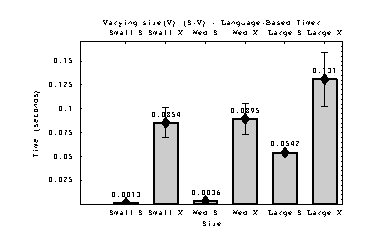
\epsfig{file=sl_chart.eps}
\vspace*{-.2in}
\begin{center}\hspace{.6in}(a)\end{center}
\end{minipage} &

\begin{minipage}{2.0in}
\centering
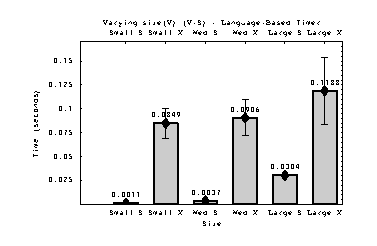
\epsfig{file=ls_chart.eps}
\vspace*{-.2in}
\begin{center}\hspace{.6in}(b)\end{center}
\end{minipage} &

\begin{minipage}{2.0in}
\centering
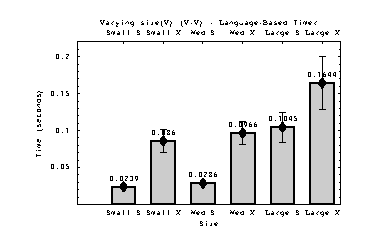
\epsfig{file=ll_chart.eps}
\vspace*{-.2in}
\begin{center}\hspace{.6in}(c)\end{center}
\end{minipage} \\

\end{tabular}

\caption{Varying {\em size(V)} for the (a) SV, (b) VS, and (c) VV Nano
Benchmarks.}

\label{fig:varying}
\vspace*{-.1in}
\end{figure*}

%% The results are significant because the
%% confidence intervals do not overlap and the result of the t-test was
%% to reject the null hypothesis.

% NOTE: This paragraph is essentially more of the same and thus I 
% am not convinced that it is really needed.  For now, I am going to 
% push a summary sentence to the previous paragraph and then remove
% all of this material.  This will save space and let us get to the
% interesting parts in the next few paragraphs.

%% Figure~\ref{fig:varying}(b) presents the results of varying $size(V)$
%% in the \texttt{VS} benchmark.  We observe that {\small
%% $R_\Delta^\%(\mbox{{\tt VS}},S_5,S_{500})$}$=2664\%$ and {\small
%% $R_\Delta^\%(\mbox{{\tt VS}},X_5,X_{500})$}$=40\%$.  The large percent
%% increase for the socket primitive can also be attributed to the low
%% response times when the {\tt VS} benchmark is used with $size(V)=5$.
%% Yet, it is important to observe that {\small $R_\Delta^\%(\mbox{{\tt
%% VS}},S_{500},X_{500})$}$=291\%$ and there are no overlapping standard
%% deviations when {\tt VS} is executed with the two primitives.  When
%% $size(V)=500$, the socket implementation had a confidence interval of
%% [0.019,0.042], while the XML-RPC primitive created a confidence
%% interval of [0.089,0.148].  Due to the fact that the confidence
%% intervals do not overlap and the result of the t-test was to reject
%% the null hypothesis, these results are significant.  This clearly
%% demonstrates that the XML-RPC primitive is slower than socket
%% communication when the {\tt VS} benchmark is executed with a maximum
%% vector size of 500.

%% Figure~\ref{fig:varying}(c) provides the results of varying $size(V)$
%% in the \texttt{VV} benchmark.  We note that {\small
%% $R_\Delta^\%(\mbox{{\tt VV}},S_5,S_{500})$}$=337\%$ and {\small
%% $R_\Delta^\%(\mbox{{\tt VV}},X_5,X_{500})$}$=91\%$.  Due to the fact
%% that socket response times are higher when {\tt VV} is executed with
%% small vectors, the percent increase for the socket primitive is
%% smaller for the {\tt VV} benchmark than for {\tt SV} and {\tt VS}.
%% Socket response times are faster than XML-RPC since {\small
%% $R_\Delta^\%(\mbox{{\tt VV}},S_{500},X_{500})$}$=57\%$ and the
%% standard deviations do not overlap when {\tt VV} is executed with the
%% two primitives. When $size(V)=500$, the socket implementation had a
%% confidence interval of [0.090,0.119] and the confidence interval of
%% XML-RPC was [0.128,0.201].  Since these confidence intervals do not
%% overlap and the t-test rejects the null hypothesis, we judge sockets
%% to have better performance than XML-RPC when {\tt VV} is configured
%% with a maximum of $size(V)=500$.

%% getSendBufferSize

%% public int getSendBufferSize()
%%                       throws SocketException

%%     Get value of the SO_SNDBUF option for this Socket, that is the buffer size used by the platform for output on this Socket.

%%     Returns:
%%         the value of the SO_SNDBUF option for this Socket. 
%%     Throws:
%%         SocketException - if there is an error in the underlying protocol, such as a TCP error.
%%     Since:
%%         1.2
%%     See Also:
%%         setSendBufferSize(int)

%% At smaller values for $size(V)$, sockets always have the performance
%% advantage in terms of time overhead.

%% The response time of the socket primitive is larger than
%% that of XML-RPC when $size(V) \leq 10000$.

%% When $size(V) = 50,000$, the experimental results clearly indicate
%% that XML-RPC has a faster response time.  For instance, we see that
%% the transmission of vectors that contain 50,000 elements and consume
%% over 900,000 bytes cause sockets and XML-RPC to incur respective time
%% overheads of approximately 18 and 2 seconds.

%% , the results in Table~\ref{tab:increasebig} suggest that sockets have
%% a slight performance edge over XML-RPC.

Table~\ref{tab:increasebig} gives the results from experiments that
increased $size(V)$ to very large values during the execution of
\texttt{VV}.  Overall, sockets are faster than XML-RPC when
$size(V)=5000$, whereas XML-RPC demonstrates a slight performance
advantage when the vectors have 10000 items.  Further analysis reveals
that {\small$R_\Delta^\%(\mbox{{\tt VV}},S_{5000},X_{5000})=$}16\% and
the two primitives have overlapping confidence intervals of
[0.292,0.304] for sockets and [0.292,0.401] for XML-RPC.  Even though
these intervals overlap, the result of the t-test was to reject the
null hypothesis and we judge that the socket primitive has better
performance.  Figure~\ref{fig:ecdf} provides an empirical cumulative
distribution function (ECDF) that explains why the two communication
primitives have different response time characteristics when {\tt VV}
is executed with $size(V)=5000$.  The ECDF curve represents the
probability that the response time is less than or equal to a specific
value on the horizontal axis.  Figure~\ref{fig:ecdf} shows that
$R(\mbox{{\tt VV}}, S_{5000})$ is always less than $.309$ seconds
while only $80\%$ of the $R(\mbox{{\tt VV}}, X_{5000})$ values fall
between $.316$ and $.35$ seconds.

%% When $size(V) = 50,000$, we see that the transmission of vectors that
%% contain 50,000 elements and consume over 900,000 bytes causes sockets
%% and XML-RPC to incur respective time overheads of approximately 18 and
%% 2 seconds.

%% scale = 5
%% 18.784 - 1.697
%% 17.087
%% 17.087/1.697
%% 10.06894
%% quit

Executing {\tt VV} with $size(V)=10000$ exposes the fact that
{\small$R_\Delta^\%(\mbox{{\tt VV}},S_{10000},X_{10000})=$}$-12\%$ and
thus XML-RPC exhibits better response times than sockets.  The
confidence intervals for sockets and XML-RPC were respectively
[0.588,0.608] and [0.469,0.577] and the result of the t-test was to
reject the null hypothesis.  Table~\ref{tab:increasebig} also shows
that the results for $size(V)=50000$ were more pronounced and thus
{\small$R_\Delta^\%(\mbox{{\tt VV}},S_{50000},X_{50000})=$}$-1006\%$.
The confidence interval for the socket implementation was
[18.078,19.490], the interval for XML-RPC was [1.616,1.777], and the
t-test rejected the null hypothesis.  These results clearly
demonstrate that the socket implementation performs worse than the
XML-RPC primitive when transmitting large parameters and return
values.  We explored a wide range of parameter settings in order to
ensure that this marked performance change was not due to an improper
configuration of sockets.

%% the {\tt java.net} library.

%% For example, when the call to {\tt setPerformancePreferences(0,1,0)}
%% was used to indicate that latency should be favored over all other
%% performance measures, this did not change the response times.

%% Yet, response times did not differ when we called {\tt
%%   setPerformancePreferences(0,1,0)} in order to indicate that low
%% latency should be favored over all other performance measures.

For instance, increasing the size of the socket server's JVM heap to
256 MB or modifying the size of the socket's send and receive buffers
with the {\tt setSendBufferSize} and {\tt setReceiveBufferSize}
methods provided by {\tt java.net.Socket} did not change the response
time results in Table~\ref{tab:increasebig}.  We also used the {\tt
  setPerformancePreferences(CON, LAT, BAN}) to modify the performance
preferences for the socket primitive and this did not change the
results for the socket-based version of {\tt VV}.  The parameters {\tt
  CON}, {\tt LAT}, and {\tt BAN} respectively indicate the relative
importance of short connection time, low latency, and high bandwidth.
Yet, response times did not differ when we called {\tt
  setPerformancePreferences(0,1,0)} in order to favor low latency over
connection time and bandwidth.

%% A cumulative distribution function (CDF) give the probability than a
%% random variable X is less that a given value x. (F(x) = Pr{X<=x}). An
%% empirical distribution function is quite similar, the only difference
%% being that we work from data rather than theorectical functions.  To
%% build an empirical distribution function:

\begin{table}[t]

  \begin{center}
  \begin{tabular}{| c | c | c | c |}
  \hline
  $size(V)$ & $size(V)$ (bytes) & $R(\mbox{\tt VV}, S)$ (sec) &  
  $R(\mbox{\tt VV}, X)$ (sec) \\  \hline
  5000  & 80,520   & 0.298 & 0.347\\
  10000 & 161,000  & 0.598 & 0.523\\
  50000 & 927,720  & 18.784 & 1.697\\
  \hline
  \end{tabular} 
  \end{center} %}

  \vspace*{-.15in}
  \caption{Response Time with Very Large Vectors.}
  \label{tab:increasebig}

\vspace*{-.2in}
\end{table}

%% \begin{figure*}[t]
%% \centering
%% \begin{tabular}{c c c}

%% \begin{minipage}{2.0in}
%% \centering
%% 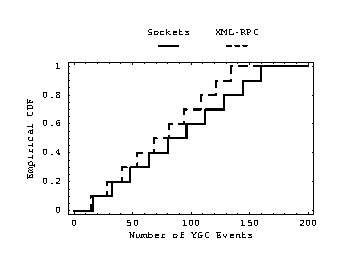
\epsfig{file=ecdf5000.eps}
%% \vspace*{-.25in}
%% \begin{center}\hspace{.2in}(a)\end{center}
%% \end{minipage} &

%% \begin{minipage}{2.0in}
%% \centering
%% 
\epsfig{file=ecdf10000.eps}
%% \vspace*{-.25in}
%% \begin{center}\hspace{.2in}(b)\end{center}
%% \end{minipage} &

%% \begin{minipage}{2.0in}
%% \centering
%% 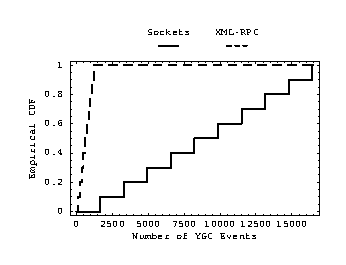
\epsfig{file=ecdf50000.eps}
%% \vspace*{-.25in}
%% \begin{center}\hspace{.2in}(c)\end{center}
%% \end{minipage} \\

%% \end{tabular}

%% \vspace*{-.1in}
%% \caption{Young GC Events for {\tt VV} and $size(V)=$ (a) 5000, (b)
%% 10000, and (c) 50000.}

%% \label{fig:jvm_behave}
%% \end{figure*}

\subsection{Virtual Machine Behavior}
\label{sec:virt-mach-behav}

%% We calculate the GC ratio in terms of the number of objects and the
%% allocation size in bytes.

This paper uses JVM behavior profiles to explain the response time
characteristics revealed in Sections~\ref{sec:time-overhead}
and~\ref{sec:variation}.  In particular, we focus on a benchmark's
heap allocation behavior and the execution of the JVM's garbage
collector.  The JVM heap is divided into several regions respectively
known as permanent, old, and young.  The young space is further
sub-divided into three regions known as eden, survivor one (S1), and
survivor two (S2).  We record the number of times the collector
performs a full collection over all three regions and a young
collection for eden, S1, and S2.  It is important to note that the
young GC (YGC) events often occur more frequently than the full GC
(FGC) events even though a full GC consumes more time overhead.

%% This paper also reports the GC object ratio for a benchmark as the
%% number of allocated objects divided by the number of live objects at
%% the point of server termination (the GC byte ratio can be calculated
%% in an analogous fashion).  A high GC byte ratio suggests that a
%% benchmark allocates and then de-allocates a significant amount of data
%% and this could cause an increase in response time.

%%  and this can also be explained by examining the JVM's behavior.

Figure~\ref{fig:realworlds} shows that the {\tt REV} benchmark takes
longer to complete when it uses XML-RPC instead of the socket
primitive.  This is due in part to the fact that the socket primitive
does not cause any YGC or FGC events to occur.  The XML-RPC primitive
forces 122 YGC events that consume .059 seconds and 5 FGC events that
increase response time by .123 seconds.  The XML-RPC server must also
perform additional string processing in order to reverse the input
vector and this increases the response time as well.
Table~\ref{tab:increasebig} shows that the execution of {\tt VV} can
yield very high response times for sockets.  Table~\ref{tab:allgc}
reveals that sockets and XML-RPC have similar GC behavior when
$size(V)=5000$ and $size(V)=10000$.  For example, S-{\tt VV} and
X-{\tt VV} both avoid a full garbage collection when 5000 objects are
transmitted.  Even though sockets do require more GC activity when
$size(V)=10000$, the YGC and FGC events only increase response time by
.073 seconds.

\begin{figure}[t]
\centering
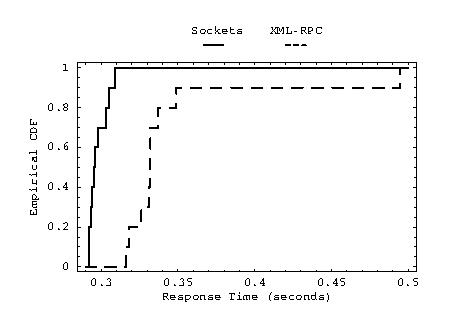
\epsfig{file=ecdf.eps}
\vspace*{-.1in}
\caption{Response Time for {\tt VV} when $size(V)=5000$.}
\label{fig:ecdf}
%\vspace*{-.1in}
\end{figure}

%% Table~\ref{tab:allocate} shows that the XML-RPC primitive has a higher
%% GC object ratio than sockets and this suggests that the XML-RPC server
%% allocates and then later collects a greater number of objects.  

%% Table~\ref{tab:allocate} shows that this heap allocation behavior
%% yields a GC byte ratio of 148.83 for sockets and 7.48 for XML-RPC.
%% While the socket primitive's GC object ratio is smaller than that of
%% XML-RPC, it has a significantly higher GC byte ratio and we judge that
%% this causes the marked increase in response time as seen in
%% Table~\ref{tab:increasebig}.

Table~\ref{tab:allgc}(a) indicates that S-{\tt VV}'s JVM performs 1645
YGC and 663 FGC events when $size(V)=50000$, while X-{\tt VV} only
causes 123 YGC and 5 FGC events.  The 10.375 seconds associated with
performing the full GC events represent $55\%$ of the execution time
for S-{\tt VV}.  In contrast, the FGC events performed by the X-{\tt
  VV} JVM correspond to $2.9\%$ of the benchmark's total execution
time.  The use of the JVM heap profiling agent called {\tt hprof}
reports that the S-{\tt VV} JVM allocates $152,539$ objects to the
heap while $1,506,476$ objects are allocated by the X-{\tt VV} JVM.
However, the S-{\tt VV} benchmark allocates $710,374,184$ bytes and
the X-{\tt VV} JVM only stores $54,101,312$ bytes.  At the point of
benchmark termination, S-{\tt VV} has $4,773,224$ bytes of live
objects in the JVM heap and the X-{\tt VV} heap contains $7,234,520$
bytes of live objects.  Finally, the JVM behavior profiles reveal that
the {\tt java.net.Socket} implementation allocates many {\tt char[]}
arrays while the XML-RPC primitive relies upon instances of the high
performance {\tt java.nio.CharBuffer}.  These results further support
the conclusion that S-{\tt VV} is slow because (i) it allocates and
subsequently collects many more bytes than X-{\tt VV} and (ii) sockets
in Java 1.5 do not take advantage of the fast character buffers in
Java's ``new input/output'' (NIO) package.

\begin{table*}[t]

\begin{center}
\begin{tabular}{|c||c|c|}

\hline
 {\bf Comparison}     &{\bf CI Sockets}     &{\bf CI XML-RPC} \\
\hline
 $R(SS,S_{5})$ vs $ R(SS,X_{5})$  & [0.17, 0.17]   & [0.269, 0.293] \\
\hline
 $R(VV,S_{5})$ vs $R(SS,X_{5})$   & [0.17, 0.17]   & [0.252, 0.328] \\
\hline
 $R(VV,S_{5})$ vs $R(VV,X_{5})$  & [0.023, 0.025]   & [0.072, 0.107] \\
\hline
 $R(REV,S_{5})$ vs $R(REV,X_{5})$  & [0.17, 0.17]   & [1.902, 2.039] \\
\hline
 $R(GRAB,S_{5})$ vs $R(GRAB,X_{5})$ & [0.17, 0.17]   & [0.159, 0.191] \\
\hline
 $R(GCD,S_{5})$ vs $R(GCD,X_{5})$  & [0.002, 0.003]   & [0.067, 0.104] \\
\hline
 $R(REV,S_{5})$ vs $R(REV,X_{5})$& [0.002, 0.004]   & [1.687, 1.834] \\
\hline
 $R(SV,S_{500})$ vs $R(SV,X_{500})$& [0.050, 0.058]   & [0.106, 0.156] \\
\hline
 $R(VS,S_{500})$ vs $R(VS,X_{500})$& [0.019, 0.042]   & [0.089, 0.148] \\
\hline
 $R(VV,S_{500})$ vs $R(VV,X_{500})$ & [0.090, 0.119]   & [0.128, 0.201] \\
\hline
 $R(VV,S_{5000})$ vs $R(VV,X_{5000})$   & [0.292, 0.304] & [0.292, 0.401] \\
\hline
 $ R(VV,S_{10000})$ vs $ R(VV,X_{10000})$   & [0.588, 0.608] & [0.469, 0.577] \\
\hline
 $ R(VV,S_{50000})$ vs $ R(VV,X_{50000})$  & [18.078, 19.490]  & [1.616, 1.777] \\

\hline
\end{tabular}
\end{center}

\vspace*{-.15in}

\caption{Summary Table for Statistical Analysis.}
\label{tab:XMLResults}

\vspace*{-.1in}

\end{table*}

\subsection{Network Resource Consumption}
\label{sec:space}

%% We also observe that the average packet size is smaller whenever the
%% socket primitive is compared to XML-RPC.

Table~\ref{tab:sover} shows the network resource consumptions for the
micro benchmarks with $size(V) = 500$.  We do not report consumption
measurements for benchmarks that were executed with large $size(V)$
values since very high data transfer rates caused the {\tt tcpdump}
kernel filter to drop a significant number of packets and this could
yield incorrect estimates for $W$.  The most obvious trend to note is
that socket communication always generates more packets than XML-RPC.
Across all benchmarks, the average number of packets received by the
GNU/Linux kernel was 7222 for the socket primitive and 380 for
XML-RPC. We also observe that the average packet size is smaller for
sockets than XML-RPC.  Considering every benchmark, the mean of the
average packet sizes is 86 bytes for the socket primitive and 802
bytes for the XML-RPC communication mechanism.

%% 4008*71.16
%% 285209.28
%% 180*861.67
%% 155100.60

An estimate of the total network resource consumption in bytes can be
made by multiplying the average size by the total number of packets
received by the kernel filter.  This estimate is not entirely accurate
since the average packet size is computed by sizing the packets that
were captured and stored for later analysis.  Further analysis shows
that {\small $W_\Delta^\%(\mbox{{\tt SS}},S,X)=$}31\%, {\small
  $W_\Delta^\%({\tt SV},S,X)=$}119\%, {\small $W_\Delta^\%(\mbox{{\tt
      VS}},S,X)=$}$-69\%$, and {\small $W_\Delta^\%(\mbox{{\tt
      VV}},S,X) =$}$-45\%$.  These percent increases suggest that
socket communication consumes fewer network resources than XML-RPC for
the \texttt{SS} and \texttt{SV} benchmarks.  As given in
Table~\ref{tab:sover}, the \texttt{VS} and \texttt{VV} benchmarks
reveal that socket communication transmits more data than XML-RPC.
For instance, we estimate that S-{\tt VS} transmits a total of 285,209
bytes whereas X-{\tt VS} only transfers 155,100 bytes during
execution.  This results suggests that, at the packet level, XML-RPC's
textual encoding of vectors can be more space efficient than the Java
serialization mechanism used by sockets.  However, since XML-RPC
frequently causes the transmission of very large packets (e.g., X-{\tt
  VV} has an average packet size of 1455.9 bytes), this primitive
might not be suitable for interactive Java applications.

%% Table~\ref{tab:sover} shows the results of space overhead for the
%% micro benchmarks with $size(V) = 500$.  The most obvious trend to note
%% is that socket communication always generates more packets than
%% XML-RPC communication.  The average number of packets received from the 
%% socket implementations is 7222 packets compared to 380 packets for the 
%% XML-RPC implementations.  

%% Another trend is that the average packet size is smaller in every case
%% with sockets compared to XML-RPC.

% NOTE: none of this content belongs here since this is RESULTS 
% ANALYSIS and this is a detail about the evaluation metric tool
% I think that I have replicated this content correctly inside 
% of the above discussion

%% For each benchmark, the \texttt{tcpdump} tool reports the number of 
%% packets received and the number of packets captured.  The packets 
%% received is the total number of packets that were encountered on the 
%% network interface.  

% NOTE: this came from the introduction section of the paper, but after
% further reflection this content does not fit nicely here

%% \item A discussion of the threats to the validity of the experimental
%%   results (Section~\ref{sec:threats-validity}), a comparison of our
%%   work to previous empirical studies (Section~\ref{sec:related-work}),
%%   and the proposal of enhancements to both the benchmarking framework
%%   and the experiment design (Section~\ref{sec:future-work}).

\subsection{Threats to Validity}
\label{sec:threats-validity}

%% Any empirical study of the performance of a distributed system must
%% confront certain threats to validity.  

Any empirical study of the performance of local-remote software
systems must confront certain threats to validity.  During the
empirical evaluation of communication primitive performance we were
aware of potential threats to validity and we took steps to control
the impact of these threats.  Threats to internal validity concern
factors that would present alternative explanations for the empirical
results discussed in Section~\ref{sec:results}.  The first threat to
internal validity is related to the potential faults within the
benchmarking framework that Section~\ref{sec:benchmark-framework}
describes.  We controlled this threat by incorporating tools and
libraries that are frequently used by practitioners, such as {\tt
  tcpdump}, {\tt capinfos}, {\tt jvmstat}, {\tt hprof}, and the {\tt
  java.net} package.  Since we have repeatedly used these tools
without experiencing errors or anomalous results, we have a confidence
in their correctness and we judge that they did not negatively impact
the validity of our empirical study.  Moreover, Allman also leveraged
tools such as {\tt tcpdump} without noticing problems that would
compromise the results \cite{allman-per}.  We also tested each
benchmark in isolation in order to ensure that it repeatedly produced
meaningful outcomes.  Finally, we controlled threats to internal
validity by using the same workstation and preventing external user
logins throughout experimentation.

Threats to external validity would limit the generalization of our
approach and the empirical results to new benchmarks and execution
environments.  The experiments in this paper only focus on the use of
four micro and macro benchmarks and the performance measurements from
these benchmarks might be different from those produced by other
micro, macro, and application-specific benchmarks.  The experiments
only evaluate sockets and XML-RPC and thus they provide no direct
insights into the behavior of local-remote systems constructed with
other communication primitives.  However, our framework supports the
integration of other benchmarks and this paper reports on the results
from using benchmarks that are similar to those that were described by
Allman \cite{allman-per}.  Another threat to external validity is
related to the fact that the experiments measure the performance of
sockets and XML-RPC in a single execution environment. This is because
the computer hardware, JVM, operating system kernel, and other
environmental factors were not varied during experimentation.  Yet, it
is our judgment that the execution environment is representative of
one that is frequently used during the development and execution of a
local-remote software application.

\begin{table*}[t]
  
  %\vspace*{.05in}

  \begin{tabular}{c}

    \hspace*{.75in}
    \begin{minipage}{3in}
  
  {\normalsize
  
  \begin{center}
  \begin{tabular}{| c | c | c | c | c |}
  \hline
  $size(V)$ & YGC Events (count) & YGC Time (sec) &  
  FGC Events (count) & FGC Time (sec) \\  \hline
  5000  & 16 & .008 & 0 & 0 \\
  10000 & 63  & .023 & 4 & .050 \\
  50000 & 1645  & .697 & 663 & 10.375 \\
  \hline 
  \end{tabular} \newline 
   \end{center} }
  \vspace{-.21in} 
  \begin{center} \mbox{} \hspace*{2.2in} (a) \end{center}

  \end{minipage} \\

    \hspace*{.75in}
    
    \begin{minipage}{3in}

      \vspace*{.1in}

	      {\normalsize
  
  \begin{center}
  \begin{tabular}{| c | c | c | c | c |}
  \hline
  $size(V)$ & YGC Events (count) & YGC Time (sec) &  
  FGC Events (count) & FGC Time (sec) \\  \hline
  5000  & 14 & .016 & 0 & 0 \\
  10000 & 27 & .022 & 1 & .020 \\
  50000 & 123 & .695 & 5 & .143 \\
  \hline 
  \end{tabular} \newline
  \end{center} }
  \vspace*{-.2in} 
  \begin{center}\mbox{} \hspace*{2.2in} (b) \end{center}

  \end{minipage}

  \end{tabular}

  \vspace*{-.1in}

  \caption{{\tt VV}'s Garbage Collection Behavior for (a) sockets and
    (b) XML-RPC.}
  \label{tab:allgc}
  
\end{table*}

% NOTE: The data in this table can be misleading and thus I think 
% that it should be removed from the paper.

%% \begin{table}[t]
  
%%   \vspace*{-.1in}
%%   \caption{GC Ratios for {\tt VV} when $size(V)=50000$.}
%%   \label{tab:allocate}
  
%%   \vspace{.05in}
  
%%   {\small
  
%%   \begin{center}
%%   \begin{tabular}{| c | c | c |}
%%   \hline
%%   Primitive & \rule{-.1in}{14pt} 
%%   $\frac{{\mbox{\em Alloc}}}{{\mbox{{\em Live}}}}$ (objects) 
%%   \rule{-.1in}{14pt} 
%%   & $\frac{{\mbox{\em Alloc}}}{{\mbox{{\em Live}}}}$ (bytes) 
%%   \rule{-.1in}{14pt}         \\[.1in]  \hline
%%   Sockets  & 2.94   & 148.83 \\ %\hline 
%%   XML-RPC  & 13.26  & 7.48   \\
%%   \hline
%%   \end{tabular} 
%%   \end{center} }

%% \vspace*{-.2in}
%% \end{table}

%% Furthermore, the multiserver operating system recently proposed by
%% Herder et al.\ adheres to a software architecture that is similar to
%% the one used for our experiments \cite{herder-microkernel}.  Finally,
%% since the benchmarks are implemented in Java and the {\em
%%   ExperimentCampaign} uses the Perl programming language, it is
%% possible to apply new or existing benchmarks in new or similar
%% environments as long as a JVM and a Perl interpreter are available.

Threats to construct validity concern whether the evaluation metrics
accurately reflect the variables that the experiments were designed to
measure.  We judge that the response time metric is defined and
measured in a fashion that will be useful to individuals who implement
applications that perform intra-node communication.  While network
resource consumption is also a valuable metric, our current tools do
not always support the accurate measurement of $W(B, P)$.  As noted in
Section~\ref{sec:evmet}, this is due to the fact that the high rates
of data transfer rapidly exhaust the kernel buffer space that is
reserved for packet capture.  Before conducting further experiments we
will attempt to control this threat to validity by modifying the
GNU/Linux kernel and/or enhancing existing packet capture tools.

\vspace*{-.1in}

\section{Related Work}
\label{sec:related-work}

The research described in this paper is connected to prior work in the
areas of the (i) implementation of communication primitives, (ii)
benchmarking of sockets and XML-RPC, (iii) benchmarking and behavior
characterization of message passing middleware, and (iv) performance
analysis of software applications implemented in Java.

% NOTE: consider adding this in depending upon length!

\subsection{Communication Primitives}
\label{sec:comm-prim-rw}

The micro-kernel is an example of an operating system whose
architecture was driven by detailed empirical evaluations of
communication primitive performance
\cite{gefflaut-sawmill,liedtke-improve-ipc,liedtke-microkernels}.
Since interprocess communication (IPC) was often the limiting factor
in micro-kernel performance, developers designed numerous benchmarks
and used response time results to guide the design of IPC protocols
\cite{hartig-micro-kernel,liedtke-improve-ipc}.  Thus, these studies
are similar to the one in this paper since we also use empirical
results to motivate the choice between primitives for intra-node
communication.  Furthermore, Bershad et al.\ propose an interesting
and efficient mechanism to support intra-node communication with
lightweight RPCs \cite{bershad-lightweight}.  While our focus is on
modern operating systems, object-oriented languages, and virtual
machines, the LRPC primitive was implemented for both (i) the Taos
operating system and the DEC Firefly multiprocessor
\cite{bershad-lightweight} and (ii) a previous version of the Mach
kernel \cite{bourassa-implementing}.  Finally, both Karger and Herder
et al.\ have developed specialized implementations and optimizations
that improve the performance of intra-node communication
\cite{tanenbaum-minix3,karger-registers}.  In contrast to these
efforts, this paper considers the evaluation of primitives that are
already in wide use, namely Java sockets and XML-RPC.

\subsection{Sockets and XML-RPC}
\label{sec:sockets-xml-rpc}

%% (iii) measurement and modeling of computer program performance, and

%% Since Allman's experiments were performed, a new GNU/Linux kernel,
%% JVM, and XML-RPC implementation have been released.

In category (ii), this paper is directly related to Allman's empirical
analysis of the socket and XML-RPC primitives \cite{allman-per}.  This
paper is different than \cite{allman-per} because it (i) reports
benchmark results with the recent versions of sockets and XML-RPC,
(ii) solely focuses on experiments where the client and server reside
on the same node, (iii) measures response time with OS and
language-based timers, and (iv) explains the results in light of JVM
behavior.  It is interesting to note that the results of this paper
contrast with those found by Allman.  Previous work suggests that
sockets and XML-RPC have similar response time characteristics for
small transactions.  However, the experiments that use larger
transactions show that sockets perform up to an order of magnitude
better than XML-RPC \cite{allman-per}.  Our experiments demonstrate
that sockets outperformed XML-RPC with smaller transactions but that
at extremely large transaction sizes XML-RPC performed significantly
better than sockets.  We judge that the conflicting performance
characterizations could be attributed to the (i) different execution
environments (e.g., kernel, OS, and JVM), (ii) different versions of
sockets and XML-RPC, and (iii) location of the client and server JVMs.
The future experimentation described in Section~\ref{sec:future-work}
will support the resolution of the differences between these two
studies.

\subsection{Performance Benchmarks}
\label{sec:middl-benchm}

In category (iii), the detailed empirical studies by Bulej et
al.\ \cite{bulej-final}, Cecchet et al.\ \cite{cacchet-ejb-perform},
and Pugh and Spacco \cite{pugh-rubis-revisit} indicate that the
analysis and characterization of middleware performance is
challenging.  Bulej et al.\ describe a new middleware benchmarking
technique called regression benchmarking (similar to software
regression testing
\cite{kapfhammer-testing-handbook,rothermel-safe,rummel-kanonizo-sac2005})
that repeatedly executes benchmarks in an attempt to identify
performance regressions in middleware \cite{bulej-final}.
Interestingly, Bulej et al.\ determine that certain complex benchmarks
such as RUBiS and TPC-W are not applicable in the context of
regression benchmarking because their execution incurs a significant
time overhead and the results are subject to mis-interpretation
\cite{bulej-final}.  Similar to the framework described in this paper,
Bulej et al.\ focus on the use of simple benchmarks that test an
isolated feature of a system.  %middleware.

Also in the context of category (iii), Sterck et al.\ evaluate the
performance of a tuple space that is a component within a framework
for performing bioinformatics computations
\cite{sterck-taskspaces-book,sterck-taskspaces}.  While Noble and
Zlateva primarily report on benchmark results for astrophysics
computations, some of their micro benchmarks also produce results that
are relevant to the use of tuple spaces in distributed systems
\cite{noble-javaspaces}.  Like this paper, Hancke et al.\ and Neve et
al.\ specifically focus on measuring the performance of JavaSpaces
through statistically guided experiments
\cite{hancke-js-overhead,neve-doe-js}.  Maassen et al.\ propose an
alternative implementation of Java RMI and conduct a series of
detailed experiments to evaluate the performance of RMI on a 32-node
Myrinet cluster \cite{maasen-java-rmi}.  Finally, Halepovic and Deters
evaluate the performance of JXTA and they observe that one limiting
factor for JXTA throughput is the amount of control data included in a
JXTA communication message \cite{halepovic-jxta}.  These papers are
all related to this paper because they also focus on the performance
evaluation of different message passing primitives for Java.

%% remote communication primitives.

\vspace*{-.1in}

\subsection{Java Performance Analysis}
\label{sec:java-perf-analys}

%% In category (iii), Jain \cite{jain-art-perform} and Lilja
%% \cite{lilja-perform} both provide excellent introductions to the art
%% and science of computer performance analysis.  

Horgan et al.'s platform-independent analysis of Java program
performance at the bytecode level \cite{horgan-measure-runtime} is
relevant to category (iv).  Furthermore, Zhang and Seltzer present an
application-specific benchmarking framework that evaluates Java
virtual machine performance in light of the behavior of a specific
application \cite{zhang-hbenchjava}.  Dufour et al.\ propose a series
of dynamic metrics that attempt to characterize the behavior of a Java
application in a platform independent fashion \cite{dufour-metrics},
while Sweeney et al.\ use hardware performance monitors to shed light
on the performance characteristics of Java programs
\cite{sweeney-hardware}.  Finally, Hauswirth et
al.\ \cite{hauswirth-profile} present different techniques that can be
used to profile and understand the behavior of Java software
applications. Each of these examples of related work could complement
the presented framework by expanding the types of benchmarks or
enhancing the analysis of the empirical results.

\begin{table}[t]

  \vspace*{.05in}
  \begin{center}
  \begin{tabular}{| c | c | c | c |}
  \hline
  Benchmark & Received & Captured &  Avg Size (bytes)\\
  \hline
  S-\texttt{SS} & 402 & 201 & 74.06\\
  X-\texttt{SS} & 360 & 180 & 108.28\\
  \hline
  S-\texttt{SV} & 1180 & 518 & 121.14\\
  X-\texttt{SV} & 400 & 200 & 782.15\\
  \hline
  S-\texttt{VS} & 13944 & 4008 & 71.16\\
  X-\texttt{VS} & 360 & 180 & 861.67\\
  \hline
  S-\texttt{VV} & 13362 & 4044 & 78.83\\
  X-\texttt{VV} & 400 & 200 & 1455.9\\
  \hline
  \end{tabular}
\end{center}

\vspace*{-.1in}

  \caption{Network Resource Consumption.}
  \label{tab:sover}
  \vspace*{-.1in}

\end{table}

\section{Future Work}
\label{sec:future-work}

In future research, we will modify and/or re-configure the GNU/Linux
kernel and the packet capture tools in order to more accurately
characterize network resource consumption.  We will also improve the
presented work by introducing multi-threaded clients and measuring
benchmark throughput.  It would also be useful to perform these same
benchmarks on different architectures and platforms in order to
determine how the execution environment impacts the performance
results.  Furthermore, we will measure message passing performance
when the client and server exist on separate machines.  When
communication occurs between non-local JVMs, it is also important to
study the performance of the primitives on congested and/or unreliable
networks.

We intend to execute long running benchmark campaigns that invoke a
series of methods on the side of the server while continuing to
collect JVM behavior profiles.  This will enable us to identify the
impact that HotSpot\texttrademark adaptive optimization has on the
performance of the communication mechanisms.  Additional research will
also investigate alternatives to socket and XML-RPC communication such
as Java-MPI \cite{getov-mpi,judd-mpi-java}, Java RMI
\cite{grosso-rmi,maasen-java-rmi}, tuple spaces
\cite{arnold-javaspace-rdb,fiedler-per,wells-linda-java-journal}, and
JXTA \cite{oaks-jxta,seigneur-jxta}.  These alternatives will be
compared to sockets and XML-RPC in order to determine how each
communication method compares to the others in terms of response time,
network resource consumption, and JVM behavior. Finally, we will
examine the impact that XML compression algorithms (e.g.,
\cite{min-xpress}) have on the message passing performance of XML-RPC.

%\vspace*{-.1in}
\section{Conclusions}
\label{sec:conclusions}

This paper describes a benchmarking framework that supports the
empirical evaluation of intra-node communication with Java-based
primitives.  The presented method yields quantitative results that
characterize how and why sockets and XML-RPC consume time overhead and
network resources.  The use of the benchmarks in a specific execution
environment yielded interesting experimental results that characterize
the strengths and weaknesses associated with sockets and XML-RPC.
Section~\ref{sec:time-overhead} reveals that, for all of the
benchmarks, socket-based communication outperforms XML-RPC when
$size(v)=5$.  Yet, the results in Section~\ref{sec:variation} point
out that when the micro benchmarks perform bulk data transfer, the
performance of sockets degrades rapidly due to increases in the number
of GC events.

Section~\ref{sec:virt-mach-behav} further interprets the response time
results in light of the behavior of the JVM's garbage collector.  An
analysis of the JVM behavior profiles shows that socket-based
communication incurs additional time overhead when it triggers a
significant number of YGC and FGC events.  Furthermore, the results in
Section~\ref{sec:space} suggest that (i) sockets generate a larger
number of packets than XML-RPC and (ii) the average packet size
created by the socket-based benchmarks is smaller than the packet size
produced by XML-RPC.  We also furnish a detailed examination of the
threats to the validity of the experiments in
Section~\ref{sec:threats-validity}.  In conclusion, the results in
this paper can serve as valuable guides when selecting Java-based
primitives for intra-node communication.  Since it is possible to
extend our framework with new benchmarks and statistical analysis
techniques, we judge that future research can continue to develop a
deeper understanding of Java's communication primitives by using these
benchmarks.

%% use these
%% benchmarks to 

%% and the benchmarking framework offers
%% the means to perform further experimentation.

%% \begin{enumerate}

%% \item Micro and macro benchmarks have shown that sockets demonstrate
%% superior performance to XML-RPC as measured by time overhead
%% (Section~\ref{sec:time-overhead}).

%% \item Benchmarks using very large vector sizes have shown that the
%% performance of sockets rapidly decreases when the size of the data to
%% be transmitted becomes larger (Section~\ref{sec:variation}).

%% \item Remote communication using sockets generates a larger number of
%% packets than remote communication using XML-RPC
%% (Section~\ref{sec:space});

%% \item The average packet size of packets created by programs using
%% socket communication is smaller than the packet size used by XML-RPC
%% (Section~\ref{sec:space}).

%% \item XML-RPC communication generates more Young GC events than socket 
%% communication at normal sizes (Section~\ref{sec:virt-mach-behav}).

%% \item Socket communication generates more Young GC events at very large 
%% sizes (Section~\ref{sec:virt-mach-behav}).
%% \end{enumerate}

% REPEATED CONTENT FROM ABOVE ...
% From these trends, we can conclude that there are situations in which
% each communication primitive has superior performance.  Sockets have
% smaller time overheads at normal data sizes and require less network
% bandwidth at small data sizes.  XML-RPC communication has better time
% overheads at large data sizes and performs better than sockets in
% network bandwidth in the majority of cases.

{\small
\bibliographystyle{abbrv}
\bibliography{sig-alternate} }

\balancecolumns

\end{document}
